\documentclass{beamer}

\usepackage{comment}
\usepackage{color}
\usepackage{listings}
\usepackage{verbatim}
\usepackage{multicol}
\usepackage{booktabs}
\definecolor{green}{RGB}{0,128,0}

\newcommand\gehcomment[1]{{{\color{orange} #1}}}
\newcommand\add[1]{{{\color{blue} #1}}}
\newcommand\remove[1]{\sout{{\color{red} #1}}}
\newcommand\codecomment[1]{{{\color{green} #1}}}
\newcommand\redcomment[1]{{{\color{red} #1}}}
\newcommand\bluecomment[1]{{{\color{blue} #1}}}
\newcommand\greencomment[1]{{{\color{green} #1}}}
\newcommand\magentacomment[1]{{{\color{magenta} #1}}}

\begin{comment}
\tiny
\scriptsize
\footnotesize
\small
\normalsize
\large
\Large
\LARGE
\huge
\Huge
\end{comment}

\begin{document}
\title{Challenge Problem}
\author{Emily Stein}
\date{\today}

%\frame{\titlepage}

%-----------------------------------------------------------------------------
\section{Description of Challenge Problem}

\subsection{Kryptonite Conceptual Model}

\begin{frame}\frametitle{Description of Kryptonite Scenario}
Challenge yourself by setting up the input deck for the ``Kryptonite Scenario.'' It features:
\begin{itemize}
  \item Problem domain: $2000 \times 1 \times 800$ m (x $\times$ y $\times$ z)
  \item Structured grid with your choice of discretization
  \item SUBSURFACE\_FLOW MODE RICHARDS
  \item Hydrostatic initial conditions
  \item Regional pressure gradient (Dirichlet boundary conditions)
  \item Extraction well
  \item Recharge (Neumann boundary condition)
  \item SUBSURFACE\_TRANSPORT
  \item Aqueous, solid, sorbed phases
\end{itemize}

\end{frame}

%-----------------------------------------------------------------------------
\frame{\frametitle{2D Kryptonite Scenario Schematic}
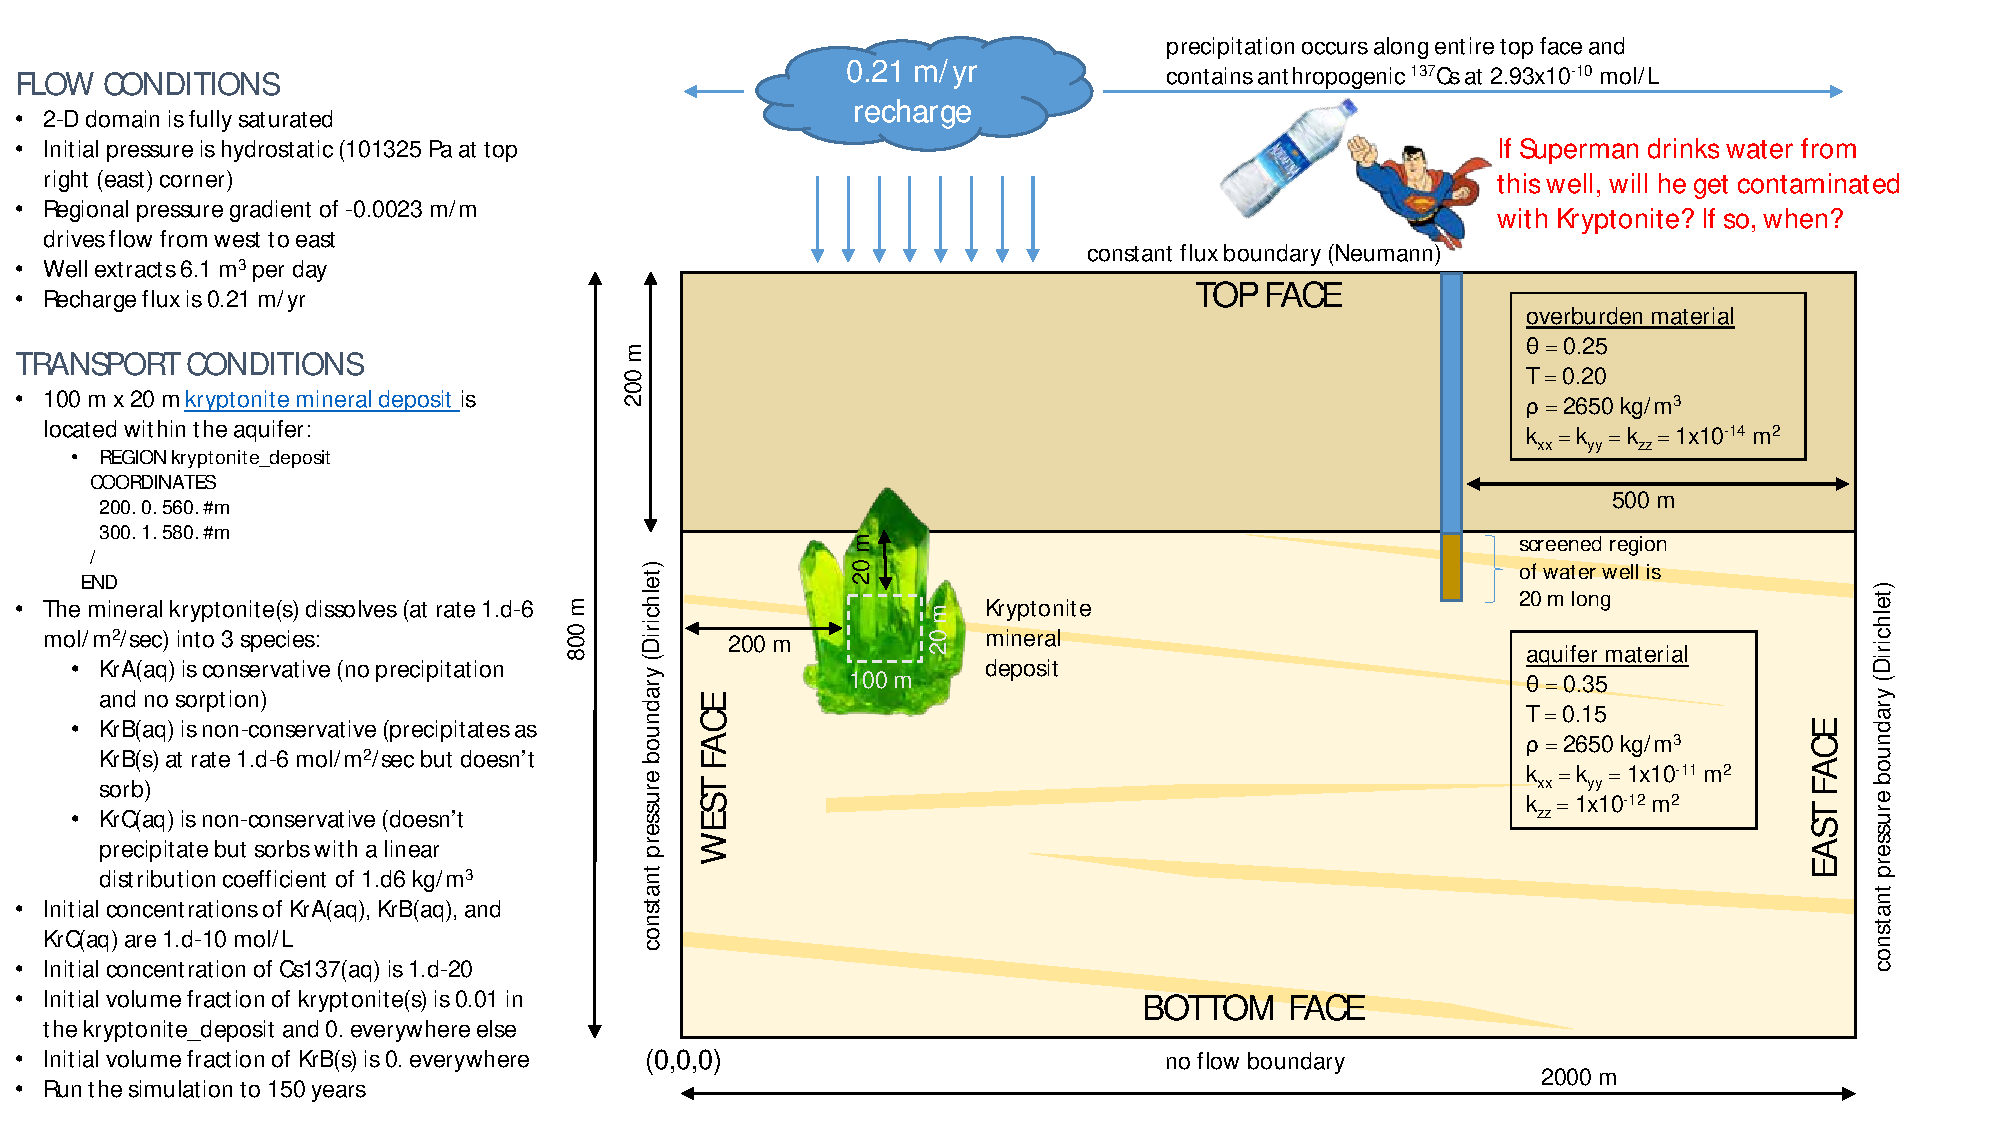
\includegraphics[width=\linewidth]{./kryptonite_schematic}
}

%-----------------------------------------------------------------------------
\section{Description of Problem}

%-----------------------------------------------------------------------------
\subsection{The Problem}

\begin{frame}[fragile]\frametitle{The Problem}
Superman drinks from a well downgradient of a kryptonite deposit. The kryptonite dissolves into three components:

\begin{itemize}
  \item At 1e-3 M, KrA(aq) will make Superman weak
  \item At 1e-3 M, KrB(aq) will make Superman very weak
  \item At 1e-3 M, KrC(aq) will bring Superman to the brink of death
\end{itemize}

\begin{itemize}
  \item Will kryptonite contaminate the well at levels Superman should avoid? 
  \item When should Superman avoid drinking water from the well if he wants to avoid damage from KrA(aq), KrB(aq), and KrC(aq)?
\end{itemize}

\end{frame}

%-----------------------------------------------------------------------------
\subsection{More Questions}

\begin{frame}[fragile]\frametitle{More Questions}
After the kryptonite deposit dissolves completely, Superman will no longer have to worry about his well water.

\begin{itemize}
  \item At what time does kryptonite(s) completely dissolve?
  \item When does the concentration of KrA(aq) at the well drop below 1e-3 M?
  \item Why does KrB(aq) remain at 1e-3 M for a longer time?
\end{itemize}

\end{frame}

%-----------------------------------------------------------------------------
\subsection{For Mere Humans}

\begin{frame}[fragile]\frametitle{For Mere Humans}
Superman isn't affected by I129(aq), but the rest of us should avoid drinking water with concentrations greater than about 1e-9 M.

\begin{itemize}
  \item When is it okay for a mere human to drink water from Superman's well?
\end{itemize}

\end{frame}

%-----------------------------------------------------------------------------
\subsection{General Hints}

\begin{frame}[fragile]\frametitle{General Hints}
Copy 1D\_Calcite/flow\_and\_tran.in to mykryptonite.in and begin editing.
\begin{itemize}
  \item \$ cp ../1D\_Calcite/flow\_and\_tran.in mykryptonite.in
  \item \$ vi mykryptonite.in \bluecomment{(or use text editor of choice)}
\end{itemize}
Avoid having to debug multiple changes at once. Make one set of changes at a time and try out your simulation.
\begin{itemize}
  \item \$ pflotran -input\_prefix mykryptonite
\end{itemize}
Put an observation point in the well and one in the kryptonite deposit. Copy kryptonite.py to mykryptonite.py and edit file paths and column numbers to plot concentrations.
\begin{itemize}
  \item \$ cp kryptonite.py mykryptonite.py
  \item \$ vi mykryptonite.py \bluecomment{(or use text editor of choice)}
  \item \$ python mykryptonite.py
\end{itemize}

\end{frame}

%-----------------------------------------------------------------------------
\subsection{BONUS 1}

\begin{frame}[fragile]\frametitle{Bonus \#1}
Time steps or grid cells that are too large introduce numerical dispersion.

\begin{itemize}
  \item Does decreasing MAXIMUM\_TIMESTEP\_SIZE change your answers?
  \item Does decreasing the size of grid cells change your answers?
\end{itemize}

\end{frame}

%-----------------------------------------------------------------------------
\subsection{BONUS 2}

\begin{frame}[fragile]\frametitle{Bonus \#2}
Play with increasing the recharge at the top boundary and decreasing the pressure gradient from west to east until Superman doesn't have to worry about his drinking water. 

\begin{itemize}
  \item What combinations of recharge and pressure gradient prevent kryptonite from reaching the well?
\end{itemize}

\end{frame}

%-----------------------------------------------------------------------------
\subsection{BONUS 3}

\begin{frame}[fragile]\frametitle{Bonus \#3}
Play with the model domain.

\begin{itemize}
  \item Use DXYZ instead of BOUNDS in the GRID block
  \item Add the third dimension to the domain by making the Y dimension 200 m and discretizing it
  \item Discretize a 1-m wide well that extends from x = 1499. to 1500. and y = 99. to 100.
  \item Don't forget to adjust the COORDINATES of REGION kryptonite\_deposit
  \item How does adding the third dimension affect concentrations at the well?
\end{itemize}

\end{frame}

%-----------------------------------------------------------------------------
\subsection{BONUS 4}

\begin{frame}[fragile]\frametitle{Bonus \#4}
Add an unsaturated zone to the initial condition.

\begin{itemize}
  \item Modify the HYDROSTATIC initial condition to create a 20 m thick unsaturated zone at the top of the model domain
  \item Hint: use the DATUM
  \item How long does the unsaturated zone persist? How does this initial condition affect concentrations at the well?
\end{itemize}

\end{frame}

%-----------------------------------------------------------------------------
\subsection{BONUS 5}

\begin{frame}[fragile]\frametitle{Bonus \#5}
Give the aquifer heterogeneous permeability.

\begin{itemize}
  \item Make the number of grid cells the same as in regional\_doublet/stochastic\_regional\_doublet.in
  \item Use a heterogeneous permeability field (in perm\_fields.h5) from that problem in MATERIAL\_PROPERTY aquifer
  \item (This domain will be large enough that running on 8 cores is preferable.)
  \item How does heterogeneous permeability affect the outcome at the well?
\end{itemize}

\end{frame}

%-----------------------------------------------------------------------------
\subsection{BONUS 6}

\begin{frame}[fragile]\frametitle{Bonus \#6}
Add a heat source to REGION kryptonite\_deposit. You choose the wattage.

\begin{itemize}
  \item Set the problem up in SUBSURFACE\_FLOW MODE TH
  \item Hint: See geologic\_disposal/gdsa.in for help with FLOW\_CONDITION and SOURCE\_SINK blocks
  \item You'll also need to change CHARACTERISTIC\_CURVES to SATURATION\_FUNCTIONS
  \item How does the heat source affect the flow solution? Can you see its effect in concentrations at the well?
\end{itemize}

\end{frame}

%-----------------------------------------------------------------------------
\end{document}
